\graphicspath{{./images/model}}
\section{Построение модели}

Целью данного этапа является построение модели <<демонстрационного стенда Умного дома>>, которая затем будет использована для определения оптимального расположения датчика температуры. В качестве платформы для моделирования был выбран COMSOL Multiphysics \cite{comsol}.


\subsection{Построение модели куба}

В начале работы было решено создать простую модель деревянного куба с ребром $1$ метр и толщиной стен $15$ сантиметров, а затем проанализировать изменение температуры внутри. Для создания физической модели использовался SolidWorks, а затем модель была импортирована в COMSOL. В COMSOL внутренность куба заполнили воздухом (куб воздуха с ребром $0.7$ м), материал стен выбран как Wood (pine).

Начальная температура стен и воздуха внутри $293$ К. Температура, действующая на внешнюю поверхность стен куба, задана по формуле:
\[300 + 50 \cdot \sin(\frac{\pi \cdot t[s]}{500}) K\]

Промоделлирован промежуток времени длиной $1000$ секунд с шагом $50$.
Были рассмотрены различные размеры сетки разбиения: Normal (Рис. \ref{cube-normal}), Fine (Рис. \ref{cube-fine}), Finer (Рис. \ref{cube-finer}) и Extra fine (Рис. \ref{cube-extra-fine}).

Ниже можно увидеть полученные результаты. На первой картинке изображена сама сетка, на второй и третьей температура в разрезе в момент 250 и 750 секунд соответственно.

\begin{figure}[H]
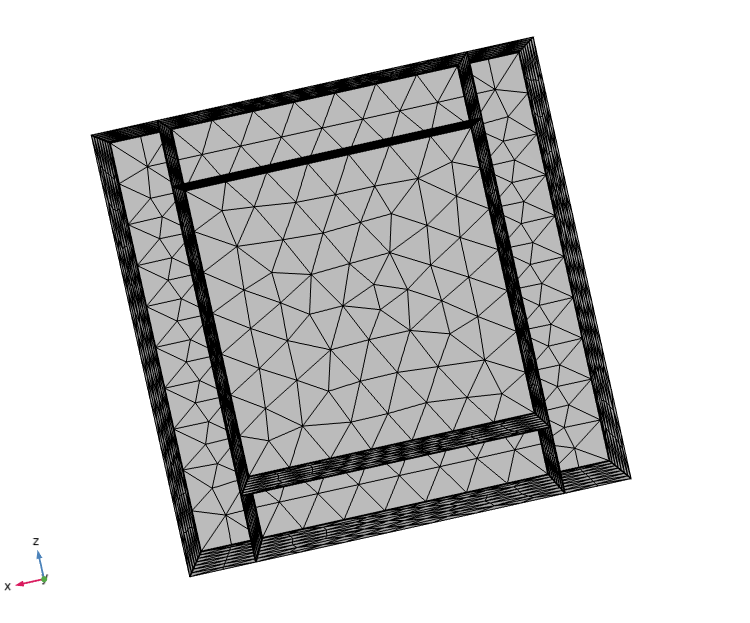
\includegraphics[width=0.3\textwidth]{cube/normal_mesh.png}\hfill
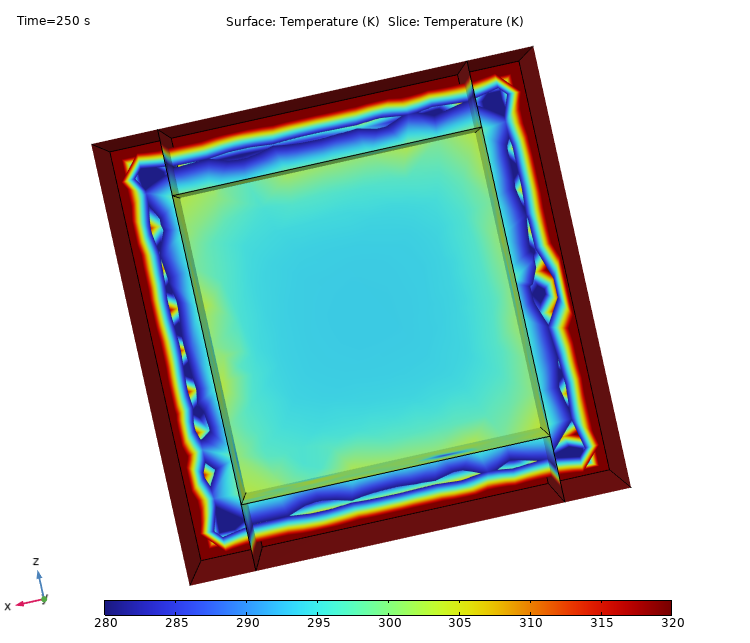
\includegraphics[width=0.3\textwidth]{cube/normal_250s.png}\hfill
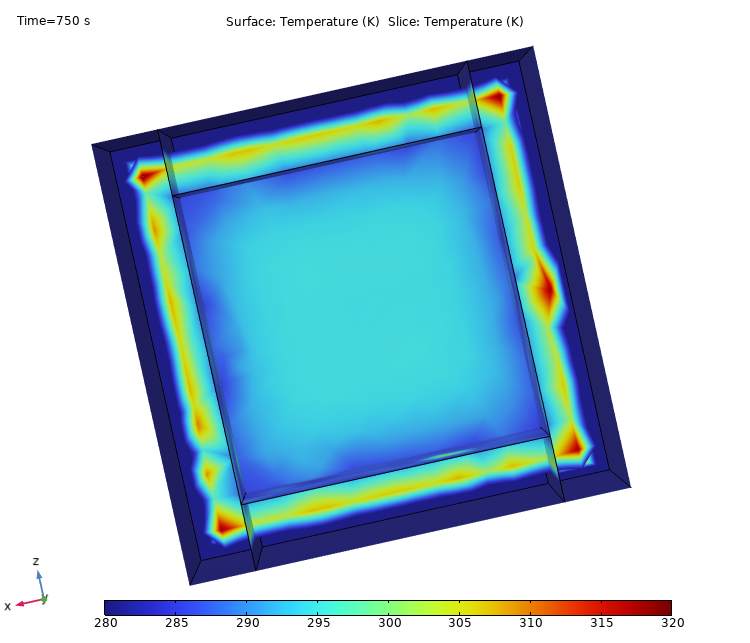
\includegraphics[width=0.3\textwidth]{cube/normal_750s.png}\hfill
\caption{Normal}
\label{cube-normal}
\end{figure}

\begin{figure}[H]
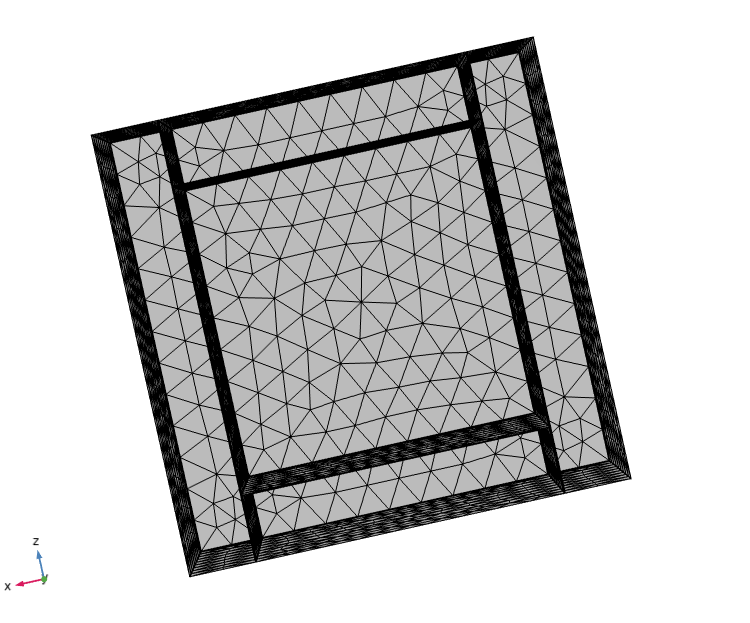
\includegraphics[width=0.3\textwidth]{cube/fine_mesh.png}\hfill
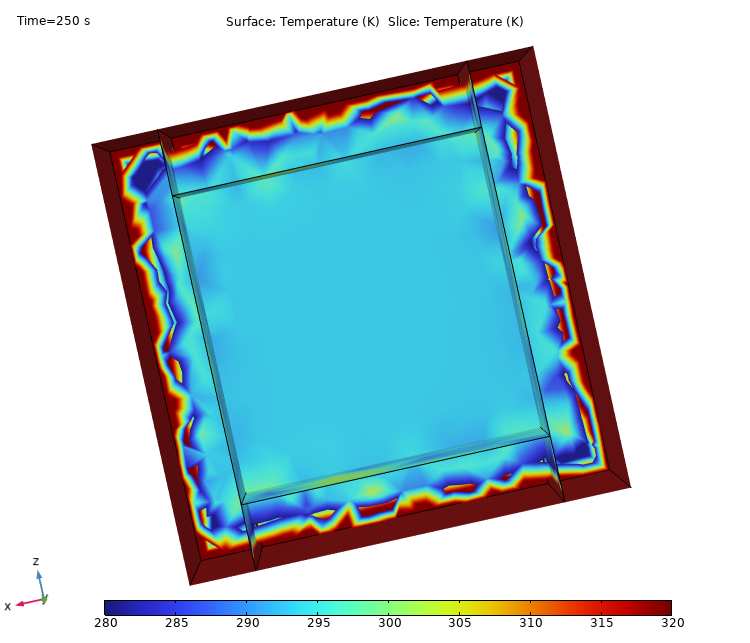
\includegraphics[width=0.3\textwidth]{cube/fine_250s.png}\hfill
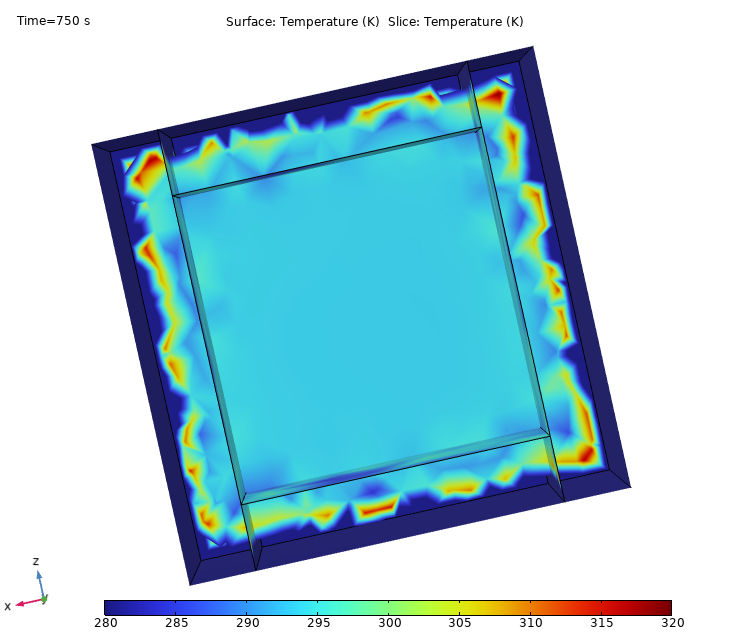
\includegraphics[width=0.3\textwidth]{cube/fine_750s.png}\hfill
\caption{Fine}
\label{cube-fine}
\end{figure}

\begin{figure}[H]
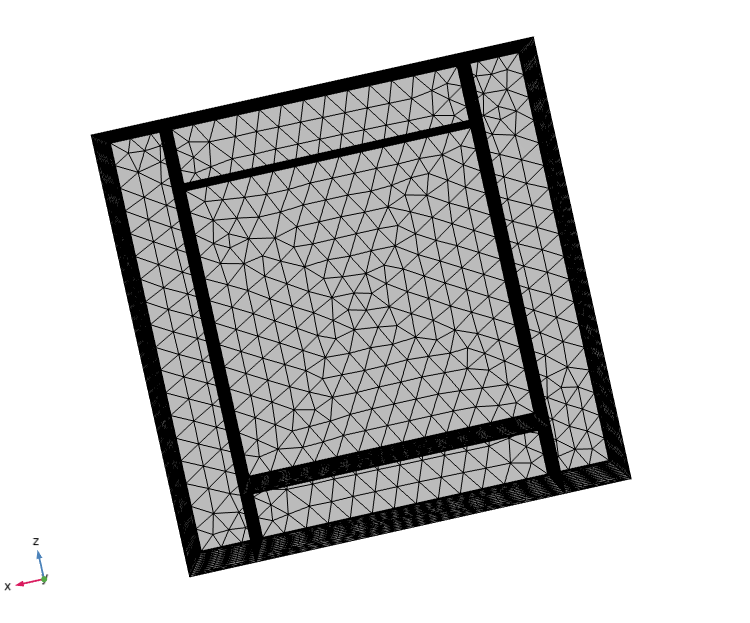
\includegraphics[width=0.3\textwidth]{cube/finer_mesh.png}\hfill
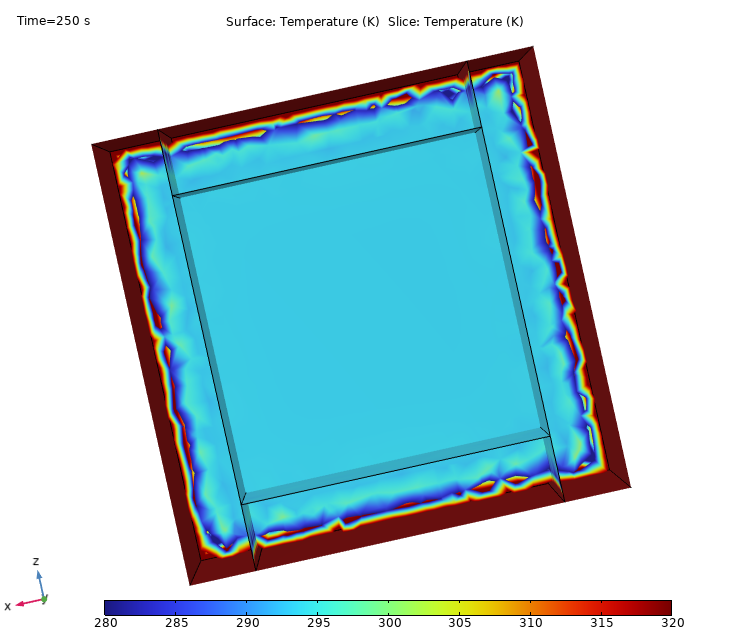
\includegraphics[width=0.3\textwidth]{cube/finer_250s.png}\hfill
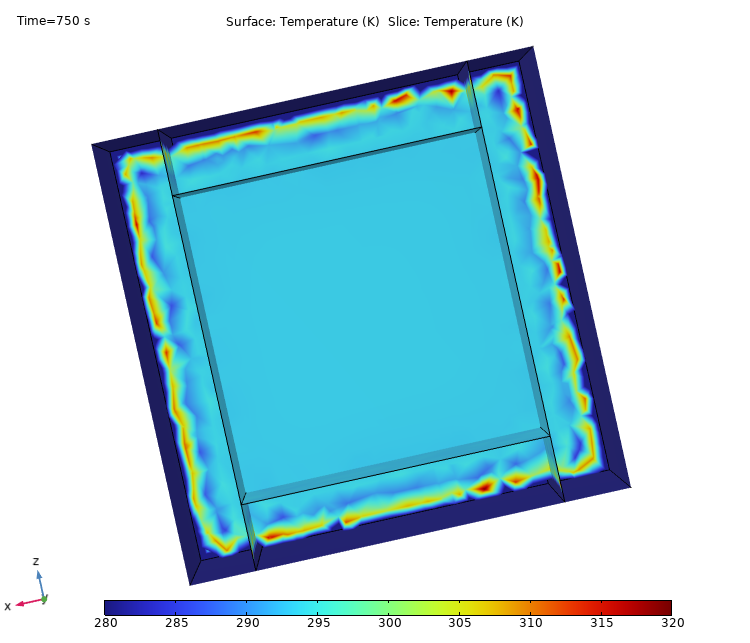
\includegraphics[width=0.3\textwidth]{cube/finer_750s.png}\hfill
\caption{Finer}
\label{cube-finer}
\end{figure}

\begin{figure}[H]
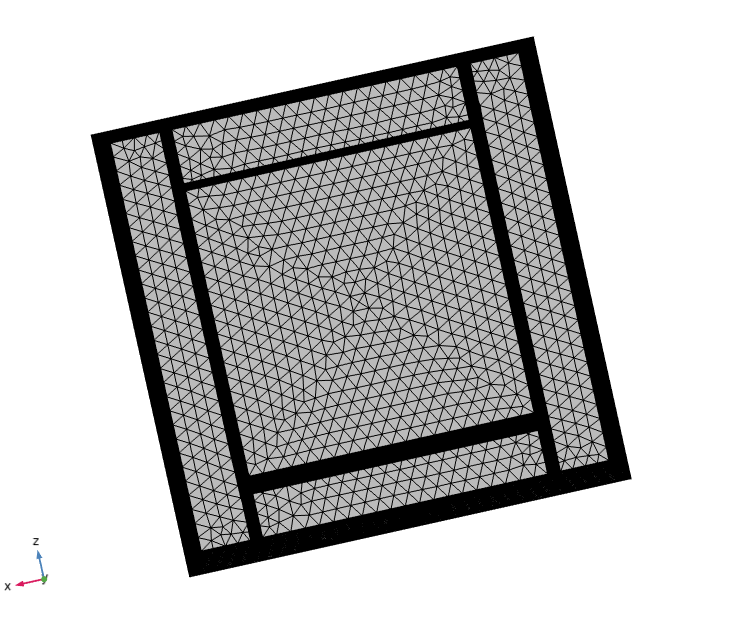
\includegraphics[width=0.3\textwidth]{cube/extra_fine_mesh.png}\hfill
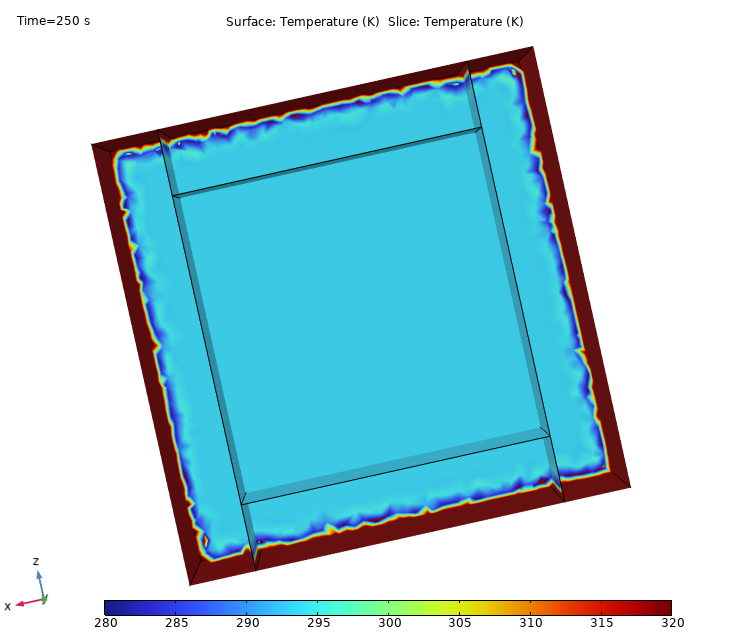
\includegraphics[width=0.3\textwidth]{cube/extra_fine_250s.png}\hfill
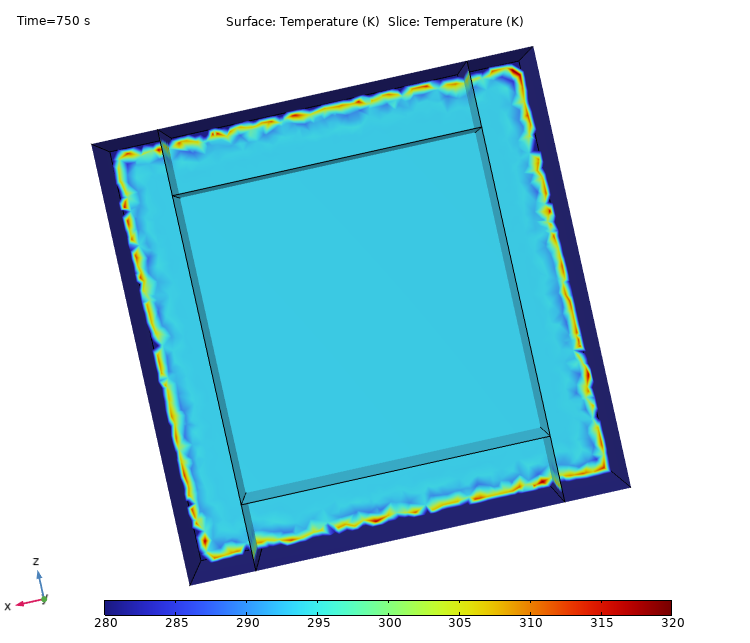
\includegraphics[width=0.3\textwidth]{cube/extra_fine_750s.png}\hfill
\caption{Extra fine}
\label{cube-extra-fine}
\end{figure}

Можно видеть, что у Normal и Fine сеток большая погрешность, тогда как начиная с Finer результат выглядит достаточно гладко. Время вычисления для Finer составило 20 секунд, для Extra fine - 80 секунд.\par
Была попытка запустить вычисления на сетке размером Extremely fine, но ожидаемое время было слишком большим и требовалось много памяти. В итоге было решено остановиться на Finer как достаточно точной при приемлемых затратах.

\newpage


\subsection{Построение модели помещения}

За основу было выбрано помещение, смоделированное в программе FreeCAD, экспортированное сначала в формат STL (но из-за особенности формата не подошло), затем в STEP (не удалось построить сетку разбиения из-за неточностей в геометрии помещения). В итоге было принято решение построить упрощенную модель сразу в COMSOL. Помещение размером $10 \times 6 \times 3 \text{ м}^3$ с окном, дверью и внутренней стеной с проходом. Материал стен - Concrete, дверь - Wood (pine), окно - Glass (quartz).

Начальная температура стен и воздуха внутри $20$ °C, внешняя температура задается синусоидой с периодом $24$ часа и амплитудой $4$ °C.
Временной промежуток $1$ день, шаг $5$ минут. Размер сетки Finer. При этом можно увидеть, что окно разбито на более мелкую сетку, чем все остальное (Рис. \ref{window}). Если отдельно сделать сетку для окна погрубее (Normal), то можно добиться снижения количества элементов разбиения на 22\% (в данном примере было $98659$, стало $76413$) без ухудшения качества.

\begin{figure}[H]
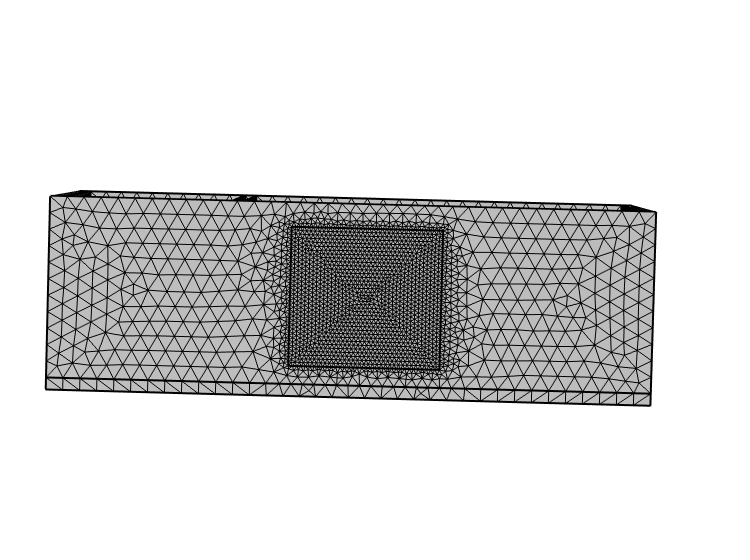
\includegraphics[width=0.5\textwidth]{smart_room/simple/window_finer.png}\hfill
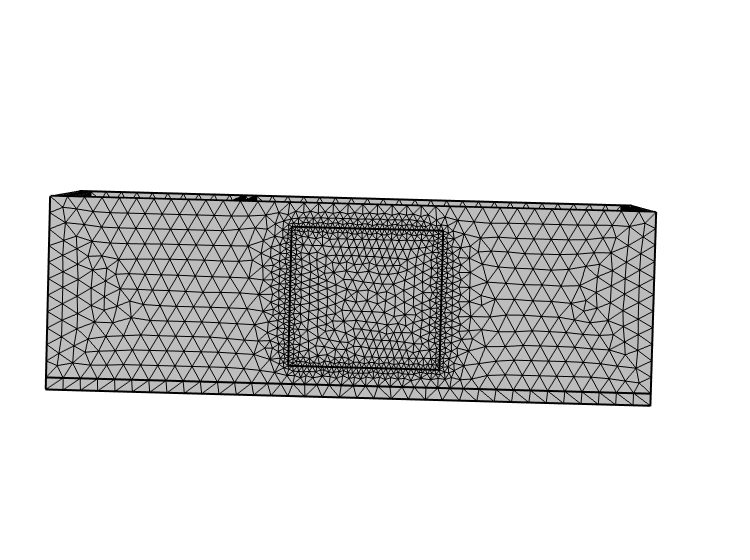
\includegraphics[width=0.5\textwidth]{smart_room/simple/window_normal.png}
\caption{Сетка разбиения окна}
\label{window}
\end{figure}


Полученные результаты можно увидеть на изображениях снизу. На них показана температура стен и температура воздуха в горизонтальном разрезе.

\begin{figure}[H]
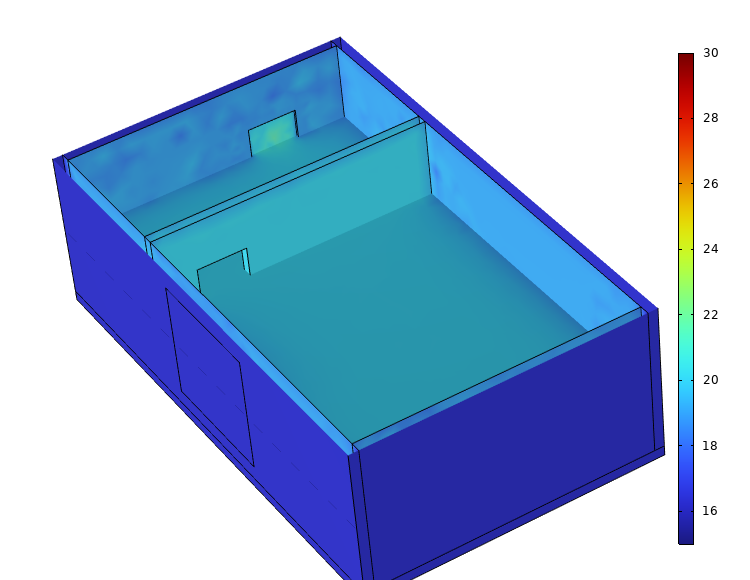
\includegraphics[width=0.5\textwidth]{smart_room/simple/finer_6h.png}\hfill
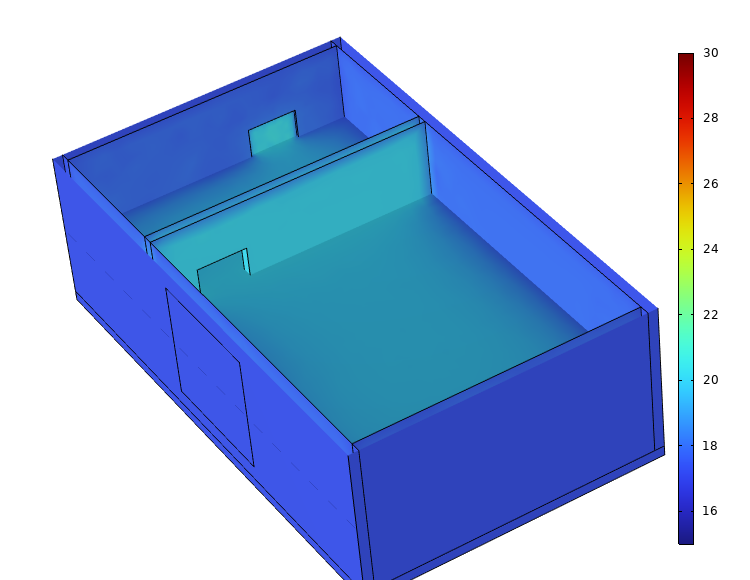
\includegraphics[width=0.5\textwidth]{smart_room/simple/finer_9h.png}
\caption{6 и 9 часов}
\end{figure}

\begin{figure}[H]
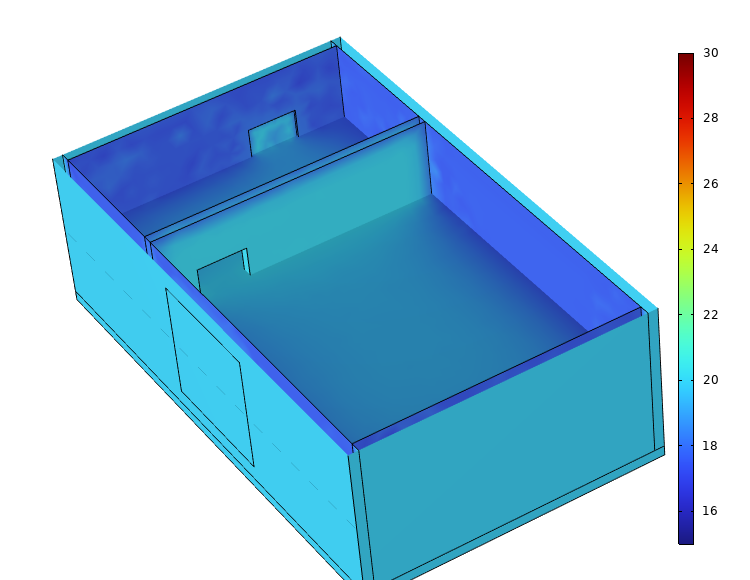
\includegraphics[width=0.5\textwidth]{smart_room/simple/finer_12h.png}\hfill
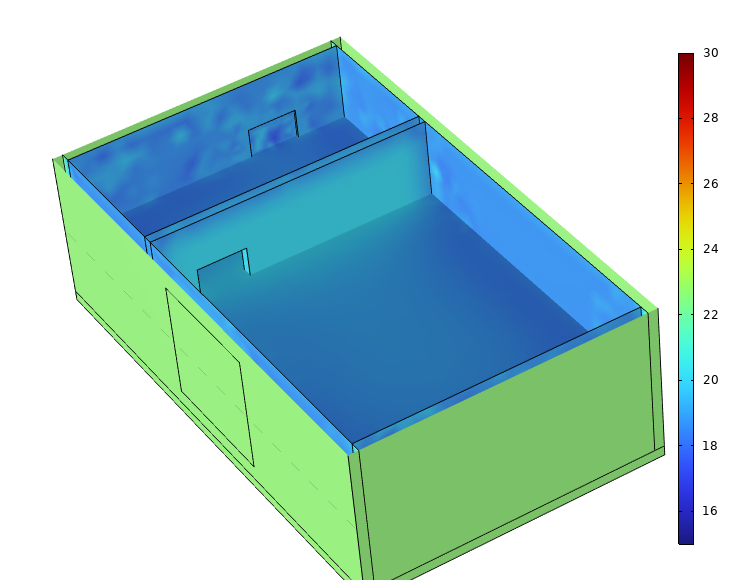
\includegraphics[width=0.5\textwidth]{smart_room/simple/finer_15h.png}
\caption{12 и 15 часов}
\end{figure}

\begin{figure}[H]
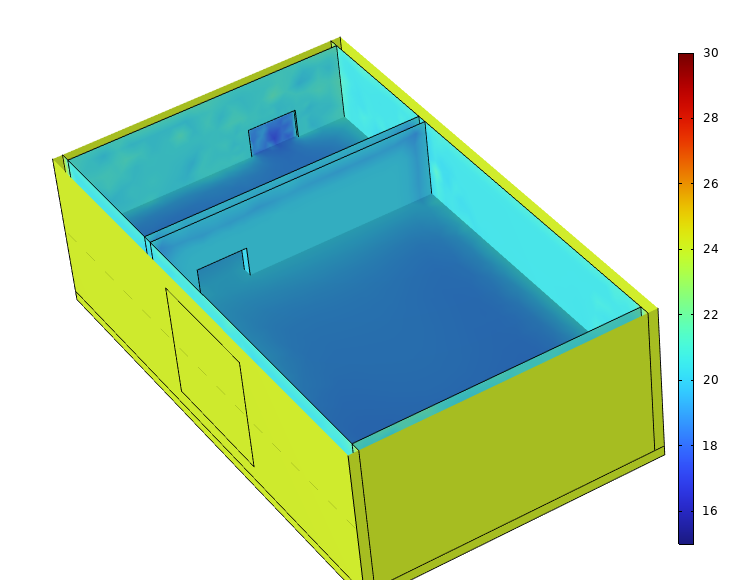
\includegraphics[width=0.5\textwidth]{smart_room/simple/finer_18h.png}\hfill
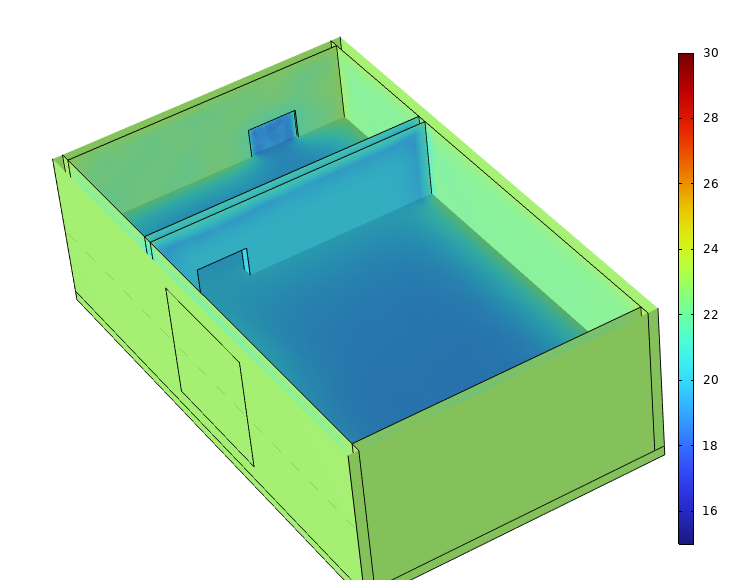
\includegraphics[width=0.5\textwidth]{smart_room/simple/finer_21h.png}
\caption{18 и 21 час}
\end{figure}
\newpage


\subsection{Моделирование с реальными данными температур}

Для моделирования погодных условий был использован датасет с температурами, использованный для прошлых исследований, за май-август 2020 года. В нем с шагом примерно 1 секунда записаны показания датчика, расположенного снаружи (Рис. \ref{real-temperature-plot}). Было решено промоделировать 4 дня с шагом в 5 минут. 

\begin{figure}[H]
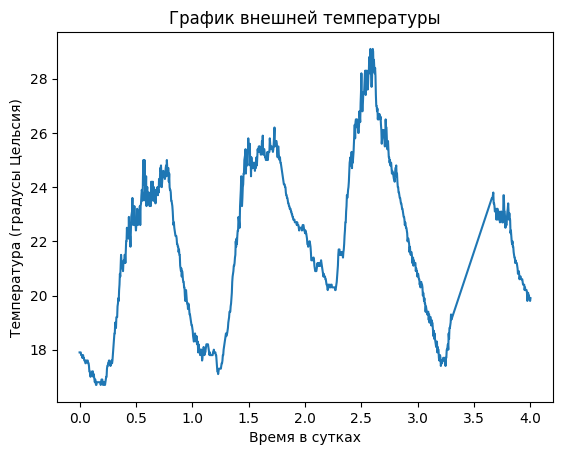
\includegraphics[width=\textwidth]{smart_room/real_temperature/temperature_plot.png}
\caption{График внешней температуры}
\label{real-temperature-plot}
\end{figure}

\newpage


\subsection{Добавление солнечной радиации}

Следующим шагом стало добавление солнечной радиации.
Все внешние стены комнаты и потолок, а также внутренние стены и пол, на которые могло светить солнце сквозь стекло, были подвержены тепловому излучению. Окно расположено стороной на юг.

В качестве источника радиации выбрано солнце, географическое расположение помещения - город Москва, дата 04.08.2020.
Полученные результаты ниже (Рис. \ref{fine-radiation}). На этих изображениях можно отметить нагрев части пола, на которую светит солнце через окно.

\begin{figure}[H]
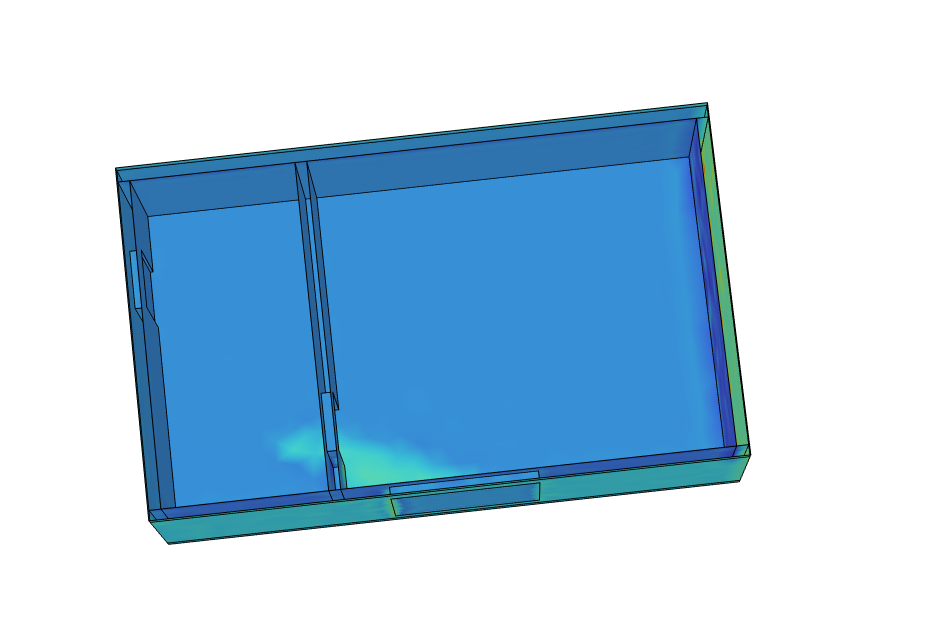
\includegraphics[width=0.5\textwidth]{smart_room/solar_radiation/fine_1.png}\hfill
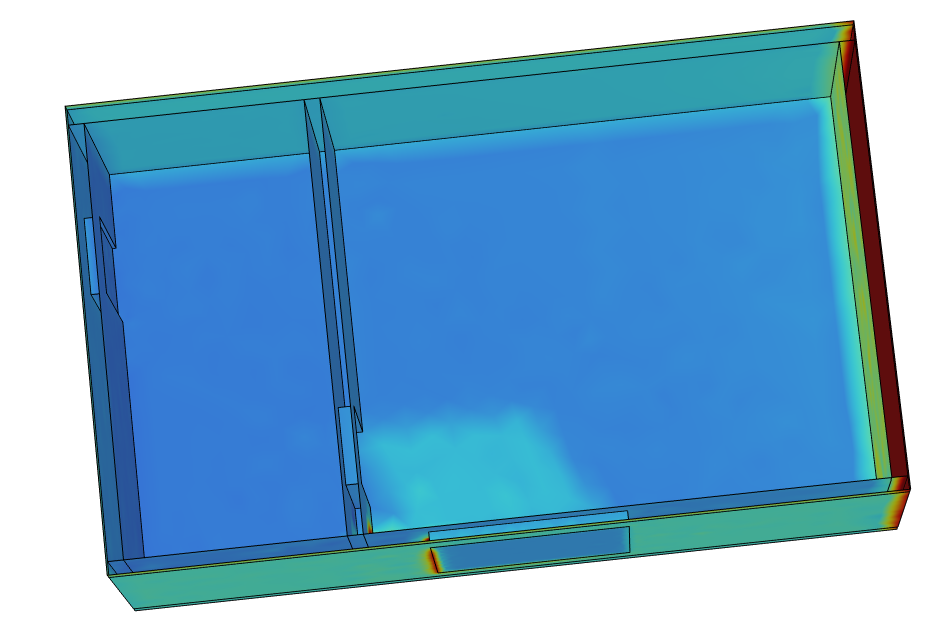
\includegraphics[width=0.5\textwidth]{smart_room/solar_radiation/fine_2.png}\hfill
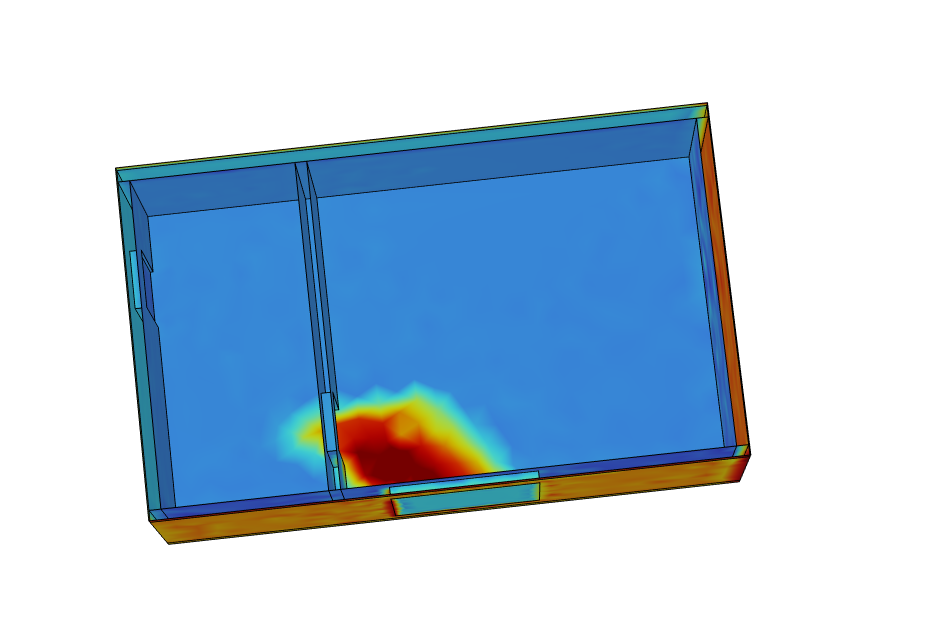
\includegraphics[width=0.5\textwidth]{smart_room/solar_radiation/fine_3.png}\hfill
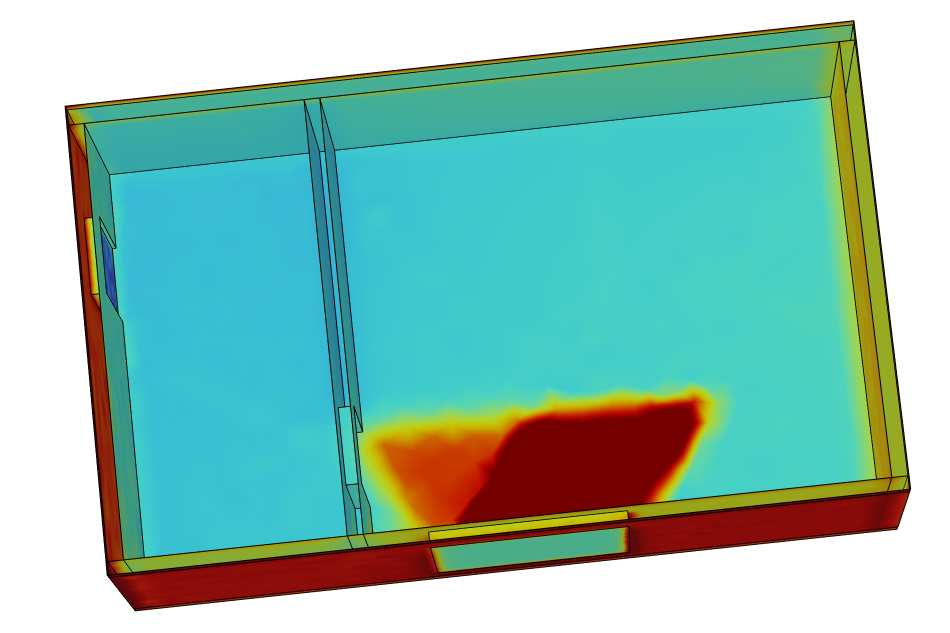
\includegraphics[width=0.5\textwidth]{smart_room/solar_radiation/fine_4.png}\hfill
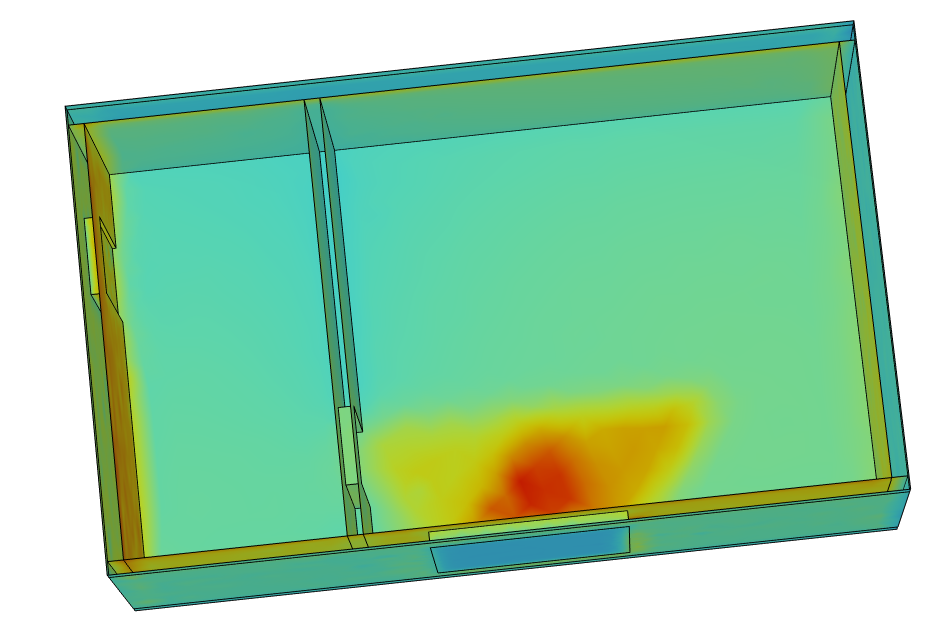
\includegraphics[width=0.5\textwidth]{smart_room/solar_radiation/fine_5.png}\hfill
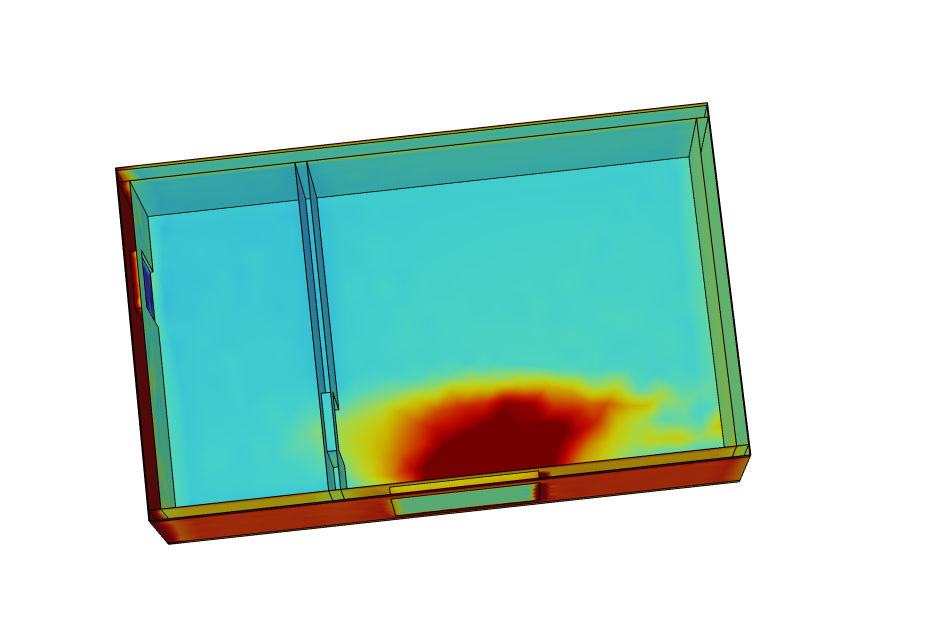
\includegraphics[width=0.5\textwidth]{smart_room/solar_radiation/fine_6.png}\hfill
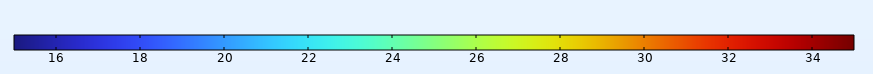
\includegraphics[width=\textwidth]{smart_room/solar_radiation/fine_color_legend.png}\hfill
\caption{}
\label{fine-radiation}
\end{figure}











































